%%%%% Elektrisches Feld %%%%%
%% #1 Beweis %%


%Some sample text to be displayed above the first subsection

%\subsection{Prinzip}

%Ein Zyklotron besteht aus Zwei hohlen, halbzylindrischen und Duanden an denen eine Spannung mit unterschiedlichem Vorzeichen anliegt, und darüber bzw. darunter liegende Magneten, die ein homogenes Magnetfeld erzeugen. Zudem gibt es einen Einlass und einen Auslass für Teilchen.

%\begin{wrapfigure}{r}{0.4\textwidth} \label{Zyklo}
%
%	\vspace{-10pt}
%	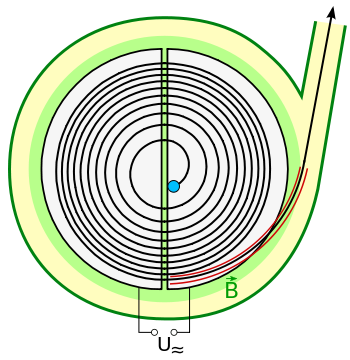
\includegraphics[width=0.35\textwidth]{Zyklotron_Prinzipskizze02.png}
%	\vspace{-13pt}
%	\caption{Prinzipskizze eines Zyklotrons}
%	\vspace{-5pt}	
%	
%\end{wrapfigure}

%\subsubsection{Anwendung}

% Some Formula:

%\begin{equation}
%	x= \frac{y \cdot 13 \pi z}
%			{\cos \alpha}
%\end{equation}

%%%%%%%%%%%%%%%%%%%%%%%
% Eigentlicher Beginn %
%%%%%%%%%%%%%%%%%%%%%%%

\subsection{Elektrostatik}

Wenn ein Körper geladen ist, bedeutet das, dass auf diesem positive und negative Ladungen in ungleich großen Mengen vorhanden sind. Daraus folgt, dass sich gleichgroße Mengen ungleichnamiger (positiv und negativ) Ladungen neutralisieren.

Gleichnamige Landungen stoßen sich ab, während ungleichnamige Ladung sich anziehen. Dies ähnelt sehr dem magnetischen Feld (Siehe \kapitelreferenz{ch:MFeld}) und steht Gravitationsfeldern entgegen, welche sich ausschließlich gegenseitig anziehen.

In Metallen sind die negativen Ladungen beweglich, sie heißen Elektronen. Diese Eigenschaft macht Metalle zu \glqq Leitern\grqq .

\begin{NiceToKnow}
Der Begriff Elektron (und alle davon abgeleitete Begriffe) kommt vom altgriechischen Wort \glqq élektron\grqq{} und bedeutet \glqq Bernstein\grqq . Der Effekt der Ladung wurde schon im alten Griechenland an Bernstein entdeckt.
\end{NiceToKnow}


\subsection{Elektroskop}	\label{subsec:Elektroskop}

Eine mögliche Bauweise eines Elektroskopes besteht im Kern aus einer Schnecke aus Metallband. Ein Zeiger, der an der Schnecke befestigt ist, schlägt aus, sobald es einen Überschuss an positiver oder negativer Ladung gibt, da sich dann durch die gleichnamige Ladungen die vielen Wicklungen gegenseitig voneinander abstoßen.


\subsection{Influenz} \label{subsec:Influenz}

Nun ist es logisch, dass bei Berührung eines Elektroskops mit einem negativ geladenen Körper, die Nadel ausschlägt, da das Metallband diese Elektronen leitet und ein Überschuss an negativer Ladung in der Schnecke zum Ausschlag führt.

Aber auch wenn ein beliebig geladener Körper (beispielsweise ein positiv geladener Kunststoffstab) nur über das Elektroskop gehalten wird, ohne es zu berühren, schlägt die Nadel aus. Dies nennt man \emph{Influenz} und das Phänomen beruht darauf, dass sich ungleichnamige Ladungen anziehen. Die beweglichen negativen Ladungen wandern durch die Anziehung des positiven Kunststoffstabs weg von der Schnecke und hinterlassen dort einen Überschuss an positiven Ladungen, sodass die Nadel ausschlägt. Entfernt man den Stab wieder, gelangt der Zeiger wieder in die Ausgangslage.

Das Besondere dabei ist, dass diese Influenz kein Medium benötigt, also auch im Vakuum über Distanzen auftritt. Damit ist ein Feldcharakter bewiesen.

\begin{Anmerkung}
Eigentlich sind nur negative Ladungen in einem Leiter beweglich, nämlich die Elektronen. Trotzdem spricht man manchmal davon, dass sich positive Ladungen von A nach B bewegen. Grundsätzlich bewegen sich dabei aber die negativen Ladungen von B nach A, sodass auf der Seite von B ein Defizit negativer Ladungen auftritt, diese Seite also positiv geladen ist.

Daher kann man von wandernden positiven Ladungen sprechen, da das Ergebnis dasselbe ist; die Mechanik dahinter ist jedoch eine Andere.
\end{Anmerkung}